\documentclass{article}
\usepackage[utf8]{inputenc}
\usepackage{titling}
\usepackage{graphicx}
\usepackage{xcolor}
\usepackage[colorlinks=true,linkcolor=darkgray, urlcolor =gray]{hyperref}
\usepackage[spanish]{babel}
\DeclareUnicodeCharacter{301}{~}
\usepackage{url}
\DeclareUnicodeCharacter{202F}{\,}


\title{Ejercicios Optativos 2}
\author{Cristina Díaz García}
\date{Diciembre 2018}

\renewcommand\maketitlehooka{\null\mbox{}\vfill}
\renewcommand\maketitlehookd{\vfill\null}


\begin{document}

\addcontentsline{toc}{section}{Índice general}

\begin{titlingpage}
\maketitle

\begin{center}

\includegraphics[scale=0.4]{images/comunicaciones.png} 
\end{center}

\end{titlingpage}

\newpage

\tableofcontents

\newpage

\section{I. Desarrollo de servicios no estándar}


\subsection{Ejercicio 2}

2. Implementar el mismo servicio de “eco” que en el ejercicio anterior pero esta vez sobre
TCP. Deberán tenerse en cuenta los siguientes requisitos de implementación:
\begin{itemize}
\item Usar la interfaz \textit{Executor} para implementar el servidor concurrente.
\item Opcionalmente implementar la otra opción de grupo de hebras y comparar ambas
implementaciones
\item El cliente le notificará al servidor el final del servicio mediante el cierre del \textit{socket}.
\end{itemize}

En este ejercicio se han implementado tres clases:

\begin{itemize}
\item \textbf{TCPCliente:} Es el cliente, al que se le pasan como argumentos al ejecutarlo, primero la dirección IP a la que conectarse, y segundo, el puerto. Si el servidor no estuviera disponible, el cliente se cierra automáticamente. En caso de que se realizara la conexión, envía y recibe los mensajes hasta que se envía un punto, en cuyo caso, el servidor cierra la conexión y el cliente se cierra.
\begin{center}
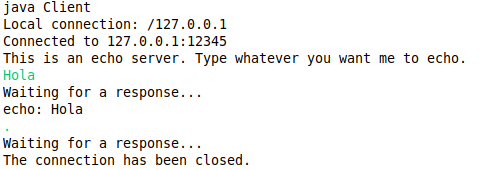
\includegraphics[scale=0.4]{images/TCPClient.png}
\end{center}
\item \textbf{TCPServer:} Es el servidor, al que se le pasa como argumento el puerto por el que escuchar. Cada vez que un cliente se intenta conectar, se crea una instancia de EchoProtocol, que es el que “gestiona” la conexión, es decir, es el que hace la función de eco.
\begin{center}
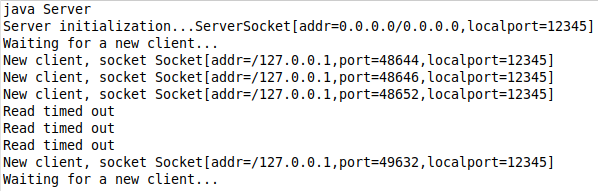
\includegraphics[scale=0.4]{images/TCPServer.png}
\end{center}
\item \textbf{EchoProtocol:} Recibe los mensajes del cliente y se los reenvía, siempre que el mensaje no fuera un punto, en cuyo caso cerraría la conexión.
\end{itemize}

Las ventajas de la implementación con TPC es la fiabilidad de la conexión. En esta implementación, uno de los problemas que tenemos es que estamos asumiendo que los argumentos se van a introducir tanto en el orden correcto como siendo los necesarios, es decir, no vamos a meter una IP incorrecta, ni vamos a introducir una palabra en vez de la IP correspondiente.

\subsection{Ejercicio 3}

3. A partir del servicio de “eco” dado en clase realizar las siguientes modificaciones para
probar las diferentes opciones de sockets sobre TCP:
\begin{itemize}
\item En el servidor, limitar el tiempo de espera de una nueva conexión dando por finalizado
el servidor tras dicho tiempo (ej: varios minutos). Nota: probar a arrancar el servidor
justo después de su finalización, antes de implementar la característica que se propone
a continuación, ¿qué ocurre?

\begin{center}
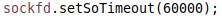
\includegraphics[scale=0.5]{images/serverTimeout.png}
\end{center}

Cuando se intenta volver a ponerlo en el mismo puerto justo después de quitarlo da un fallo al hacer binding en el puerto. Una vez que se activa, se puede volver a usar ese puerto.

\item En el servidor establecer la opción de reutilización del puerto para facilitar el arranque del servidor tras su finalización por el temporizador.

\begin{center}
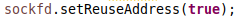
\includegraphics[scale=0.5]{images/reuse.png}
\end{center}

\item En el servidor, limitar el tiempo total del servicio de “eco” (ej: un minuto)

\begin{center}
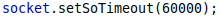
\includegraphics[scale=0.5]{images/timeout.png}
\end{center}

\item Cambiar en el cliente el tamaño del buffer de escritura a 512 bytes y comprobar si se
ha cambiado visualizando el valor anterior y el nuevo.

\begin{center}
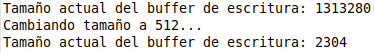
\includegraphics[scale=0.5]{images/tam.png}
\end{center}

El tamaño mínimo es 2304, por lo que no se ha podido poner a 512.

\item Deshabilitar el algoritmo de Nagle, que es especialmente recomendado si se va a
realizar el eco a nivel de caracteres o mensajes muy pequeños.

\begin{center}
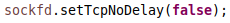
\includegraphics[scale=0.5]{images/nagle.png}
\end{center}

\end{itemize}

\section{III. Patrones de diseño}

\subsection{Ejercicio 1}

Implementar un multi-servidor que proporcione al menos dos servicios sencillos, ambos
sobre TCP. Nota: pueden ser dos versiones diferentes del servicio de “eco”.

\begin{center}
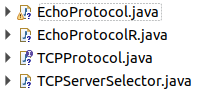
\includegraphics[scale=0.5]{images/III1.png}
\end{center}

Los dos servicios implementados, ambos implementados sobre TCP, son un servicio de eco otro de eco reverse, que devuelve invertido el mensaje invertido.
Un problema a tener en cuenta es el tener que guardar como mínimo una de las dos Keys del ServerSocketChannel para poder diferenciar los servicios para poder responder a la hora de realizar el accept, ya que al aceptarlo se crea otro SocketChannel hay que guardar su clave para poder identificar cuál es el servicio que debe hacer read o write.

\subsection{Ejercicio 2}

Implementar un servidor multi-protocolo que proporcione el servicio de “eco” sobre TCP y
sobre UDP en el mismo puerto usando el paquete NIO (Selector). El servicio de “eco” es el
mismo que el propuesto en los ejercicios I.1 y I.2. Se valorará el grado de modularización de
la solución presentada.

\begin{center}
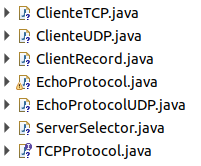
\includegraphics[scale=0.5]{images/III2.png}
\end{center}

Los clientes usados son los mismos que en los ejercicios del primer apartado, ya descritos previamente.

El servidor tiene tanto ServerSocketChannel como DatagramChannel. Le asigna al DatagramChannel un objeto de tipo ClientRecord y se registran en el selector, guardando la clave del DatagramChannel. Se crean las dos clases, tanto el echo sobre TCP como el echo sobre UDP, y con un Iterator se recorren las claves. Accept solo se usa con las claves de TCP, así que no habría que compararlas pero en Read y Write sí hay que filtrar por clave, al
guardar la clave UDP se compara esta con la obtenida en el iterator y se realizan las
operaciones de TCP o las de UDP.

El echo sobre TCP crea un SocketChannel asignado al Accept de la clave y se
registra un nuevo canal de lectura, en Read se consigue el canal de lectura de la clave y se lee en éste. Si al leer la longitud es -1 es que no hay nada y se ha cerrado la conexión. En Write se vuelve a obtener el canal de la clave y se manda el mensaje que se había leído en el buffer al cliente y por lo tanto una vez acabada la escritura vuelve a Read.

El echo sobre UDP obtiene el canal de la clave al ejeccutar el Read, y el ClientRecord asignado a esta al hacer Receive con el buffer guarda la dirección del cliente. Si esta no es
nula, se pasa a escritura, en Write se obtiene el DatagramChannel de la clave, y el
ClientRecord. Para enviar se manda el contenido del buffer a la dirección almacenados en el
ClientRecord, y se devuelve a leer.

\end{document}